\documentclass{standalone}

\usepackage{xcolor}
\usepackage{graphicx}
\usepackage{tikz}

\usetikzlibrary{shapes.geometric, arrows}
\usetikzlibrary{calc,positioning}

\graphicspath{{../../}}

\begin{document}
\nopagecolor
\large
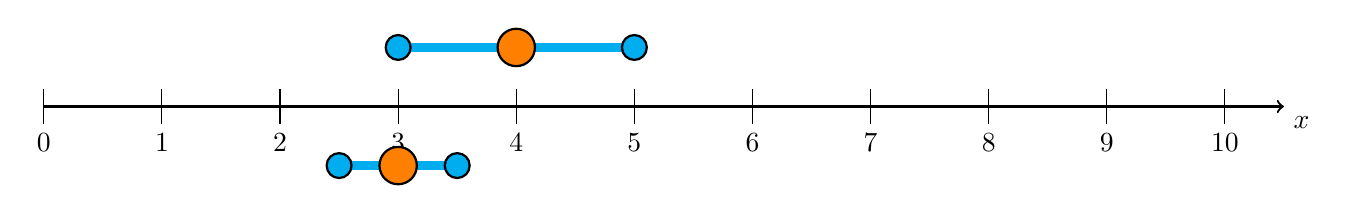
\begin{tikzpicture}[scale=1.5]

    % As
    \draw[->, thick] (0,0) -- (10.5,0);
    \node[below right] at (10.5,0) {$x$};

    % Ticks
    \foreach \x in {0,1,2,3,4,5,6,7,8,9,10} {
        \draw (\x,-0.15) -- (\x,0.15);
        \node[below] at (\x,-0.15) {\x};
    }

    \draw[line width=3pt, cyan] (3,.5) -- (5,.5);

    \draw[fill=cyan, thick] (3,.5) circle (3pt);
    \draw[fill=cyan, thick] (5,.5) circle (3pt);
    \draw[fill=orange, thick] (4,.5) circle (4.5pt);

    \draw[line width=3pt, cyan] (2.5,-.5) -- (3.5,-.5);
    \draw[fill=cyan, thick] (2.5,-.5) circle (3pt);
    \draw[fill=cyan, thick] (3.5,-.5) circle (3pt);
    \draw[fill=orange, thick] (3,-.5) circle (4.5pt);

\end{tikzpicture}
\end{document}
